\subsection{The Perturbed MNIST Dataset}

To characterise model prediction accuracy degradation as a function of added noise, we use a method similar to the work of \cite{hendrycks2019benchmarking}.

Through trial and error, parameter values were found for each perturbation function such that as the perturbation level increases from 1 to 10, the network predictive accuracy decreases from 98.52\% maximum to 36.32\% minimum, with average accuracy dropping from 97.61\% (level 1) to 48.83\% (level 10). The accuracy degradation can be observed in both Figures \ref{fig:Accuracy_vs_Noise_types} and \ref{fig:Pixelation_Digit_5_images_histogramsx10_plus_softmax}.

\begin{figure}[h!] 
\begin{center}
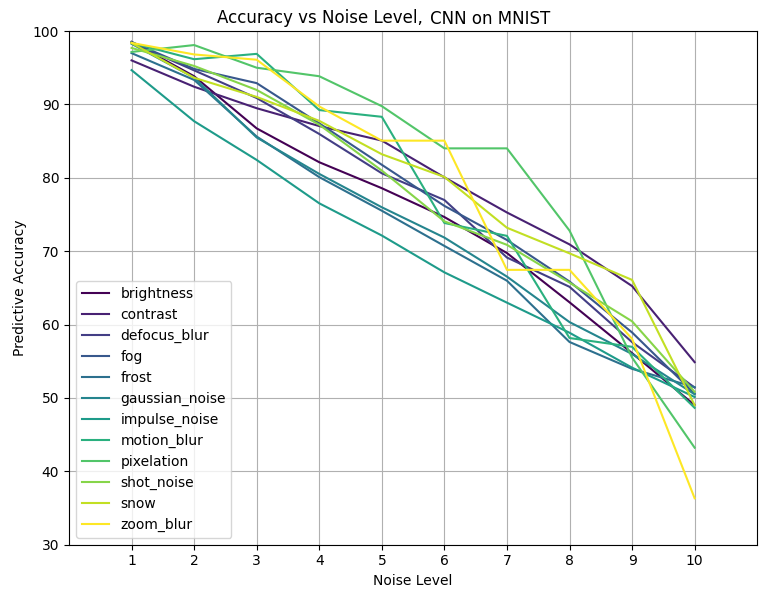
\includegraphics[width=0.99\columnwidth]{Figures/Results/Figures_accuracy_vs_noise_types_plot.png}
\end{center}
\caption{Plot for network accuracy degradation for individual perturbation types: Brightness, Contrast, Defocus Blur, Fog, Frost, Gaussian Noise, Impulse Noise, Motion Blur, Pixelation, Shot Noise, Snow and Zoom Blur.}
\label{fig:Accuracy_vs_Noise_types}
\end{figure}

Figure \ref{fig:Pixelation_Digit_5_images_histogramsx10_plus_softmax} shows digit class 5 subject to increasing levels of pixelation from left to right. The bottom row of the figure shows the average softmax output for all perturbation types at a given level. We note that at all levels from 1 to 10, the highest prediction is digit class 5 (sixth column from left to right on every plot, the first being for digit 0).
\begin{figure*}[h!]
    \centering
    
\includegraphics[width=0.99\textwidth]{Figures/Results/Figures_Pixelation_Digit_5_images_histogramsx10_plus_softmax.png}   %\captionsetup{justification=raggedright,singlelinecheck=false}
    \caption{Top row: MNIST class digit 5 subject 1 to 10 levels of pixelation going left to right. Bottom row: the average softmax output for the perturbed MNIST dataset class digit 5 for each perturbation level across all perturbation types. The change in bar heights is an indication of how images are moving closer and further to centroids in the cluster as noise increases.}\label{fig:Pixelation_Digit_5_images_histogramsx10_plus_softmax}
\end{figure*}

% generated with function call visualize_accuracy_heatmap(accuracy_matrix, perturbation_types, intensities)
\begin{figure*}[h!]
    \centering
    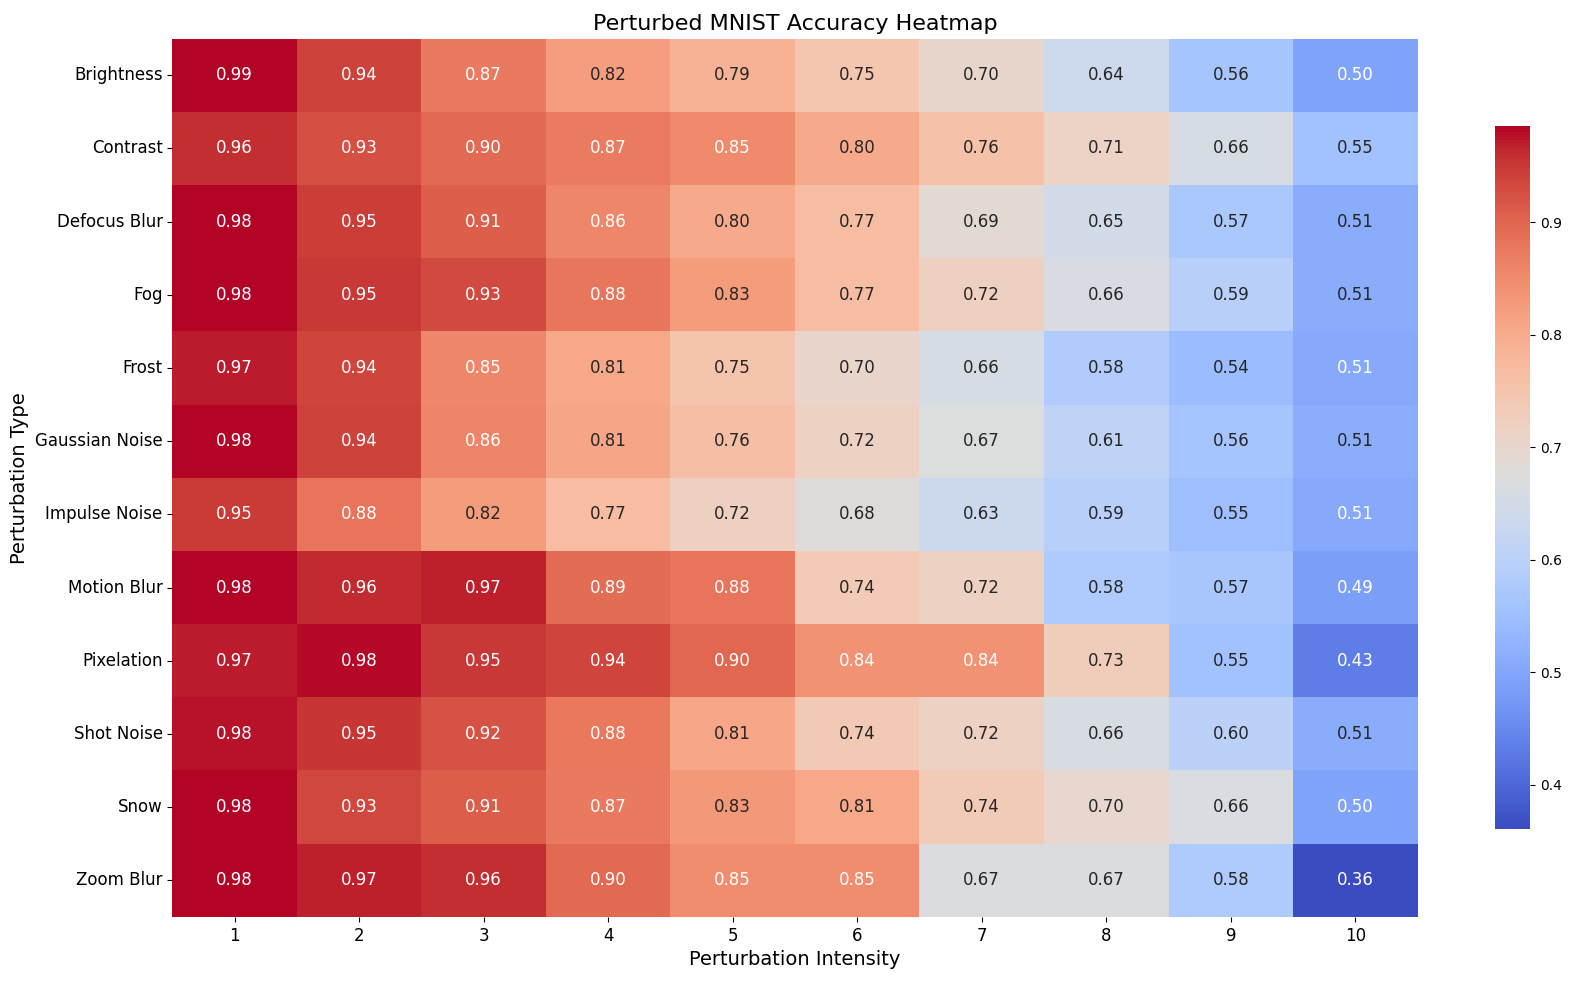
\includegraphics[width=0.99\textwidth]{Figures/Results/Figures_PerturbedMNISTAccuracyHeatmap.png}   %\captionsetup{justification=raggedright,singlelinecheck=false}
    \caption{Perturbed MNIST Accuracy Heatmap, where the accuracies are for all digit classes, given a perturbation type and intensity.}
    \label{fig:PerturbedMNISTAccuracyHeatmap}
\end{figure*}

Figure \ref{fig:PerturbedMNISTAccuracyHeatmap} shows a heatmap where every cell represents one perturbation type (y-axis, 12 total) at one intensity level (x-axis, 10 total) applied to the 10,000-image MNIST test dataset. The perturbed images are presented to the trained model and the resulting accuracy is placed in the corresponding cell. The heatmap therefore represents 1,200,000 predictions on perturbed images.

The heatmap uses a color scale from red to blue, with red indicating higher accuracy values and blue representing lower accuracy. As the perturbation intensity increases, the accuracy decreases for all perturbation types.

\begin{figure*}[h!]
    \centering
    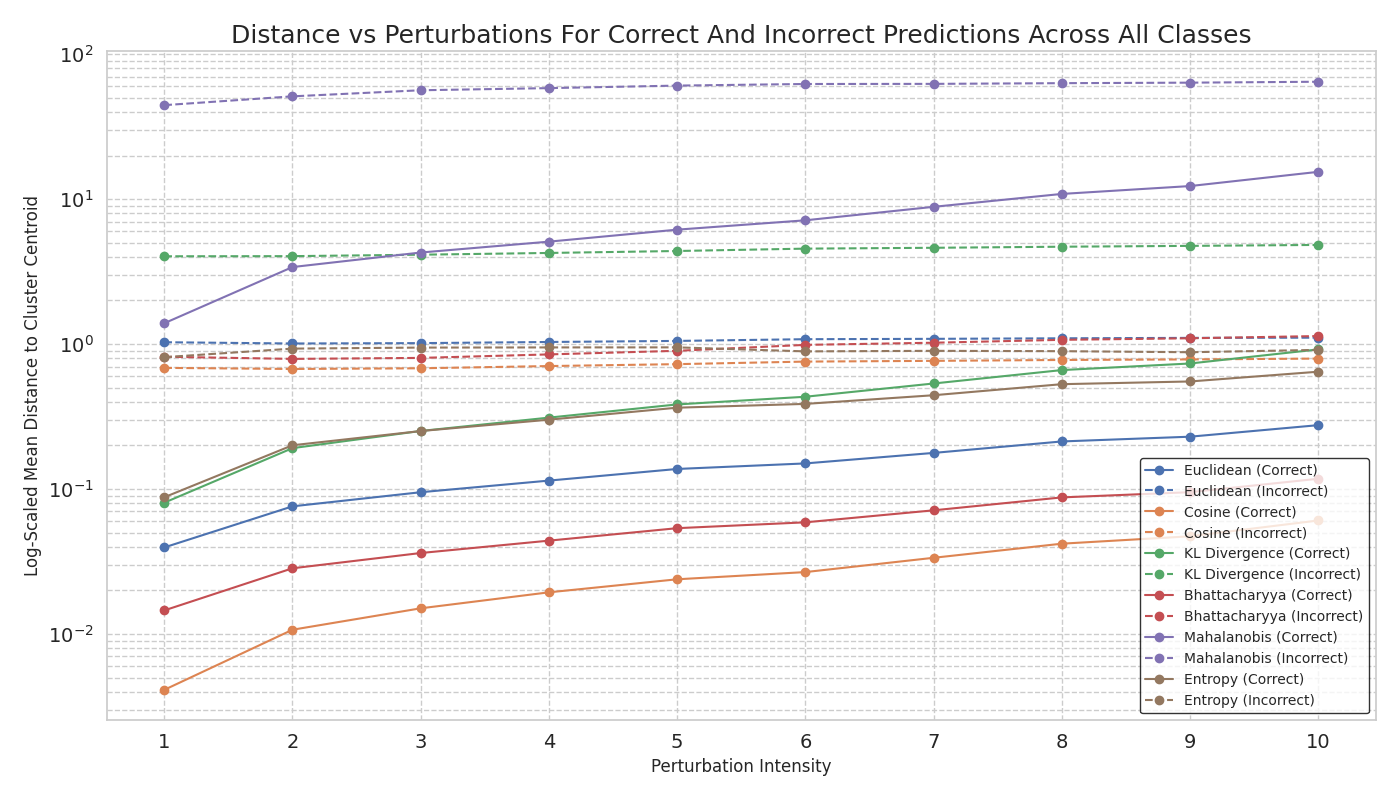
\includegraphics[width=0.99\textwidth]{Figures/Results/Figures_uncertainty_metrics.png}
    \caption{Comparison of correct vs. incorrect predictions across six distance metrics (log-scale). Solid lines represent correct predictions, dashed lines represent incorrect predictions.}
    \label{fig:Figures_uncertainty_metrics}
\end{figure*}

Figure \ref{fig:Figures_uncertainty_metrics} shows the average distance to class centroids across all classes and all perturbations for noise levels 1 through 10, comparing correct (solid line) and incorrect (dashed line) predictions for six distance metrics: Euclidean Distance, Cosine Similarity, KL Divergence, Bhattacharyya Distance, Mahalanobis Distance, and Entropy.

The plot shows that Cosine Similarity obtains maximum separation between correct and incorrect classifications, while Entropy obtains the minimum separation. Euclidean Distance proves not to be optimal; Cosine Similarity and Bhattacharyya Distance separate correct and incorrect classifications by nearly two orders of magnitude in low noise regimes and above one order of magnitude in high noise regimes, while Euclidean Distance separates by approximately one and a half orders of magnitude in low noise regimes and under one order of magnitude in high noise regimes.

The distance to centroids for correct predictions (solid lines) increases approximately linearly with perturbation intensity across all measures. The incorrect prediction distances (dashed lines) also increase with perturbation intensity but are less pronounced given the logarithmic y-axis scale. The separation between correct and incorrect predictions is important, as greater separation implies higher certainty in the decision space.

Most distance measures show good separation between correctly and incorrectly classified examples, with the exception being Entropy, which at the highest perturbation intensity presents the least separation. While Euclidean distance was selected for this study, these results suggest that alternative metrics, particularly Cosine Similarity, may provide better performance in future work.